\documentclass{standalone}
\usepackage{tikz}
\usepackage{filecontents}
% gitgraph.txt contains raw output of: $ git log --graph --oneline
\begin{filecontents}{gitgraph.txt}
* d764b48 added plaintext version in markdown
* 54ba4b2 release 2014-01-25
*   c589395 Merge branch 'master'
|\
| * 9f9c652 Remove holdover from kjh gh-pages branch
* | b3bd158 exclude font files
|/
* 63268c1 micro-typography
\end{filecontents}

\newcommand\commit[2]{\node[commit] (#1) {}; \node[clabel] at (#1) {\texttt{#1}: #2};}
\newcommand\ghost[1]{\coordinate (#1);}
\newcommand\connect[2]{\path (#1) to[out=90,in=-90] (#2);}

\begin{document}
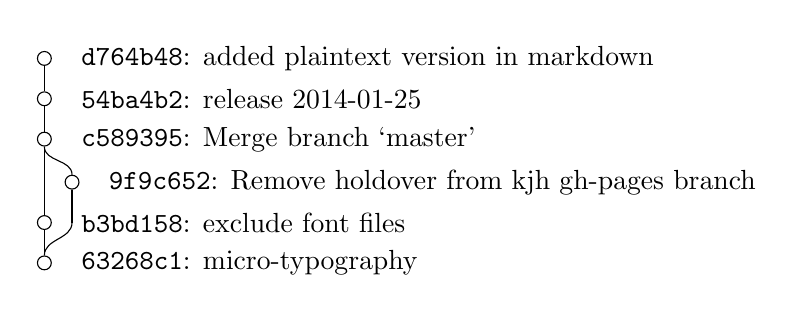
\begin{tikzpicture}
\tikzstyle{commit}=[draw,circle,fill=white,inner sep=0pt,minimum size=5pt]
\tikzstyle{clabel}=[right,outer sep=1em]
\tikzstyle{every path}=[draw]
\matrix [column sep={1em,between origins},row sep=\lineskip]
{
\commit{d764b48}{added plaintext version in markdown} & \\
\commit{54ba4b2}{release 2014-01-25} & \\
\commit{c589395}{Merge branch `master'} & \\
 & \commit{9f9c652}{Remove holdover from kjh gh-pages branch} \\
\commit{b3bd158}{exclude font files} & \ghost{branch1} \\
\commit{63268c1}{micro-typography} & \\
};
\connect{63268c1}{b3bd158};
\connect{63268c1}{branch1};
\connect{branch1}{9f9c652};
\connect{b3bd158}{c589395};
\connect{9f9c652}{c589395};
\connect{c589395}{54ba4b2};
\connect{54ba4b2}{d764b48};
\end{tikzpicture}
\end{document}
